\section{Geometric Control and Mechanics}

\begin{frame}
	\frametitle{Geometric Mechanics}
	
	\begin{itemize}
		\item Introduced by:
		\begin{itemize}
			\item F. Bullo and A. Lewis, 2005. \footcite{bulloBook}
			\item T. Lee, 2008. \footcite{Lee2008ComputationalGM}
			%\footcite{Taeyoung Lee, Computational geometric mechanics and control of rigid bodies}
			\item T. Lee et al. 2018. \footcite{LeeModel} 
		\end{itemize}
	
	\end{itemize}
	\begin{itemize}
		\item Rotating rigid body dynamics equation:
	\end{itemize}	
	\begin{equation}
		m \ddot{\textbf{x}} + m g\textbf{e}_3 = f\text{R}\textbf{e}_3 \label{model1}
	\end{equation}
	\begin{equation}
		\text{J}\dot{\mb{\Omega}} + \mb{\Omega} \times \text{J}\mb{\Omega} = \textbf{M} \label{model2}
	\end{equation}
	\begin{equation}                       
		\dot{\text{R}} = \text{R}\widehat{\mb{\Omega}} \label{model3}
	\end{equation}
	
\end{frame}

\begin{frame}
	\frametitle{Geometric Control (1)}

	\begin{itemize}
		\item PD control with nonlinear terms
		\item First developed by T. Lee et al. 2010. \footcite{LeeClanak4}
		\item Robust variant by T. Lee et al. 2011. \footcite{LeeClanak3}
		\item L1 Aadaptive controller by Kotaru et al. 2019. \footcite{Kotaru2019GeometricLA}
		\item Parameter tuning optimization by S. Lee et al. 2019. \footcite{Lee 2019}
	\end{itemize}
\end{frame}

\begin{frame}
	\frametitle{Geometric Control (2) \footcite{Markovic2019}}
	
	\begin{columns}
		\begin{column}{0.5\textwidth}\centering
			\begin{figure}[H]
				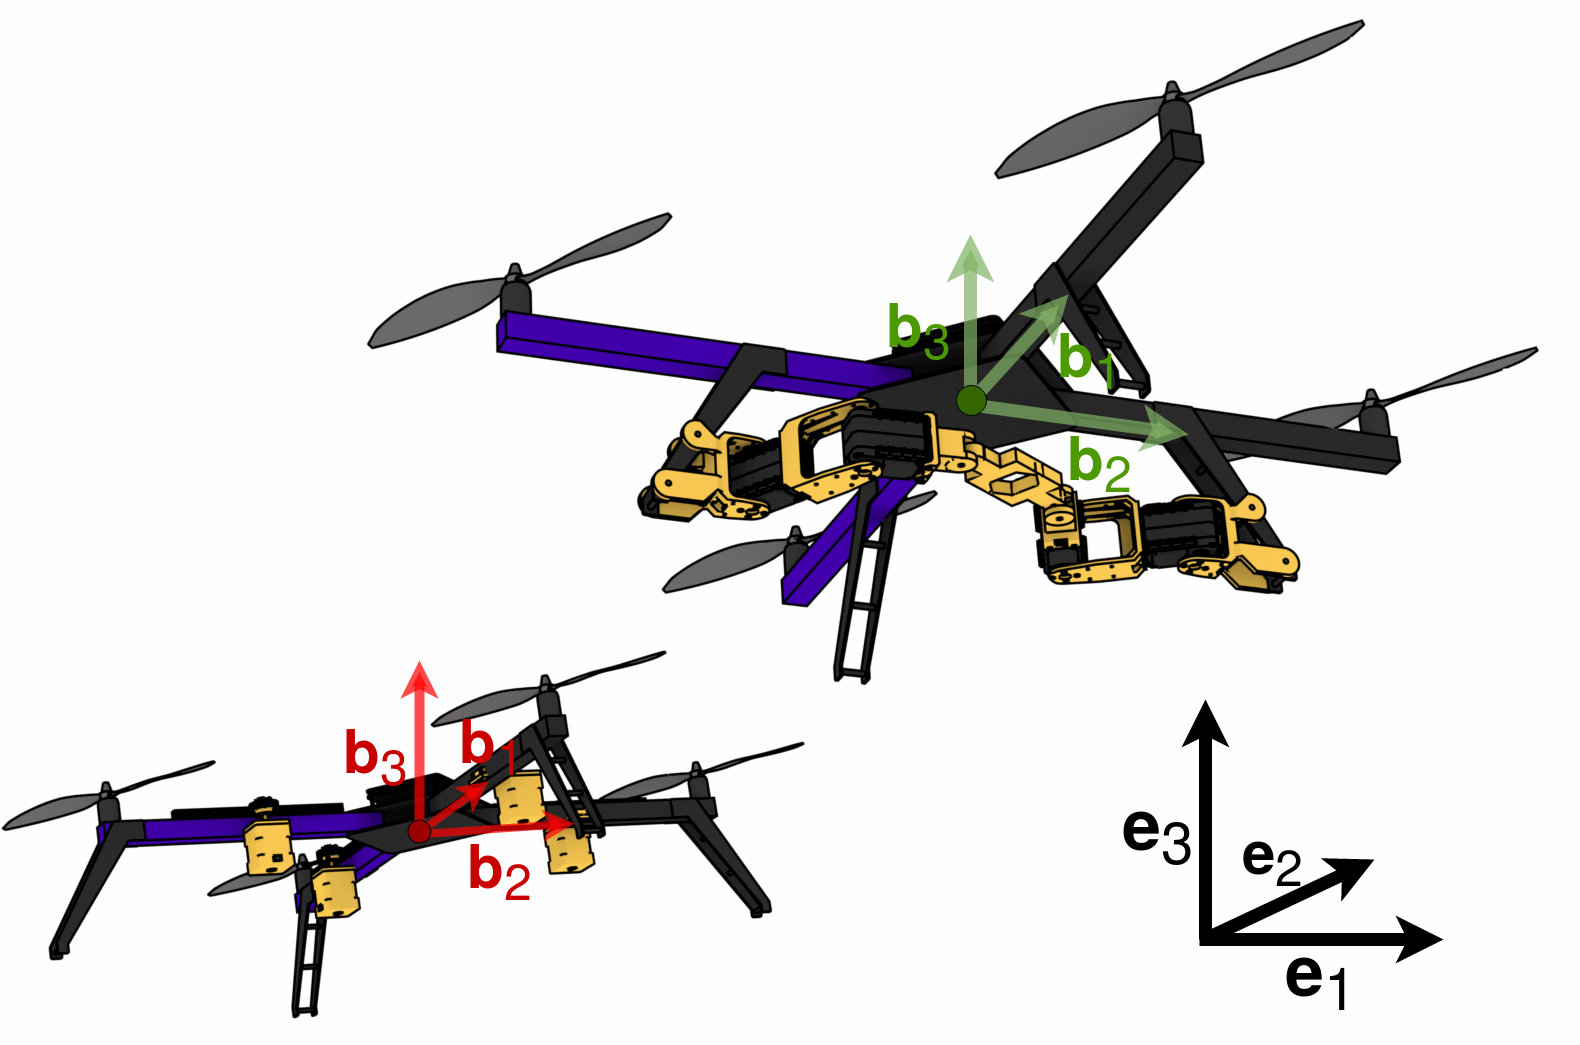
\includegraphics[width=0.8\columnwidth]{figures/uav.png}	
				\centering
				\caption{Two UAVs endowed with variable moving masses (left) and manipulator carried payload (right). }
				\label{fig:uav_model}
			\end{figure}
		\end{column}
		
		\begin{column}{0.5\textwidth}\centering
			\begin{figure}
				\centering
				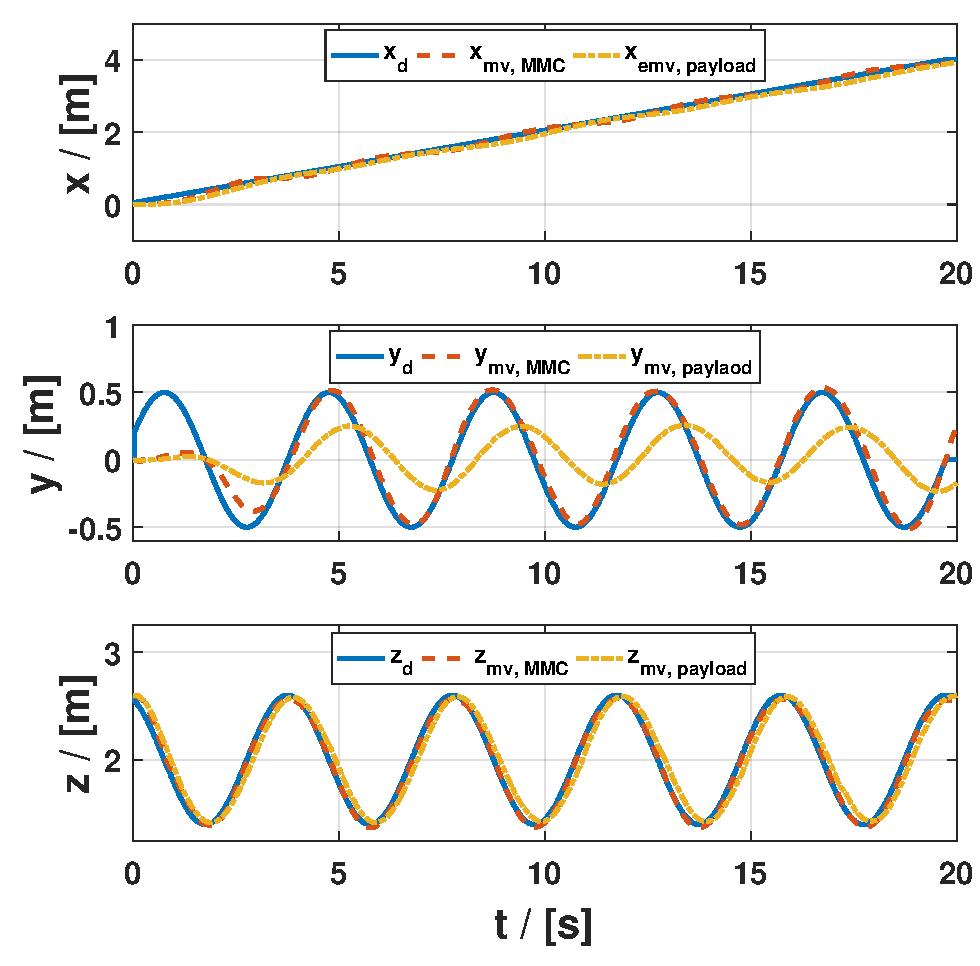
\includegraphics[width=0.95\columnwidth]{figures/both_pos_crop.pdf}
				\label{fig:traj_pos}
			\end{figure}
		\end{column}
	\end{columns}
\end{frame}